\documentclass{standalone}
\usepackage{tikz,graphicx}
\usetikzlibrary{shapes,arrows,calc,positioning,backgrounds,plotmarks,plothandlers,fit}


\begin{document}

%\begin{tikzpicture}
%  \node[draw,rectangle] (A1) {$a_{1}$};
%  \node[draw,rectangle, below of=A1] (A2) {$a_{2}$};
%  \node[below of=A2] (ellipses) {$\vdots$};
%  \node[draw,rectangle, below of=ellipses] (An) {$a_{n}$};
%
%  \node[draw,rectangle, right= of A1] (GA1) {$GA$};
%  \node[draw,rectangle, right= of A2] (GA2) {$GA$};
%  \node[below of=GA2] (ellipses2) {$\vdots$};
%  \node[draw,rectangle, right= of An] (GAn) {$GA$};
%
%  \coordinate[right of = GA1] (rGA1);
%  \coordinate[right of = GA2] (rGA2);
%  \coordinate[right of = GAn] (rGAn);
%
%  \node[draw, rectangle, right= of rGA2] (result) {routes};
%
%  \node[above = of GA1] (lthreads) {Threads};
%  \node[above = of A1] (lagents) {Agents, $\mathcal{V}$};
%
%
%  \draw[->] (A1) -> (GA1);
%  \draw[->] (A2) -> (GA2);
%  \draw[->] (An) -> (GAn);
%
%  \draw[->] (GA1) -> (result);
%  \draw[->] (GA2) -> (result);
%  \draw[->] (GAn) -> (result);
%
%
%  \draw[thick,<->] (rGAn) -> node[left] {\tiny Shared Array} (rGA1);
%
%
%  \node[draw=red, fit=(GA1) (GAn) (rGAn)]  {};
%  \node[draw=blue, fit=(A1) (An)]  {};
%
%
%\end{tikzpicture}

\begin{tikzpicture}[level/.style={sibling distance = 200cm/#1,
  level distance = 18cm}]
  \node [] {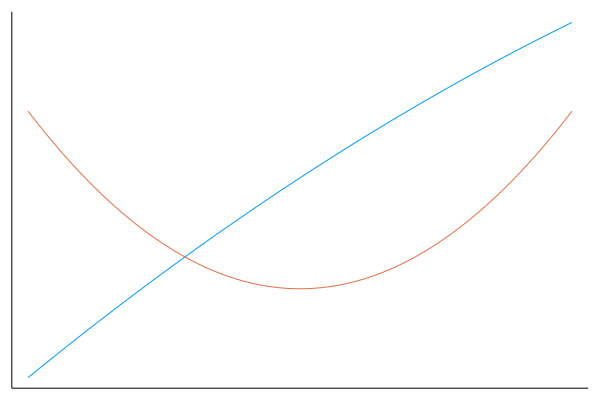
\includegraphics[]{images/bezint-1.png}}
  child{
    node [] {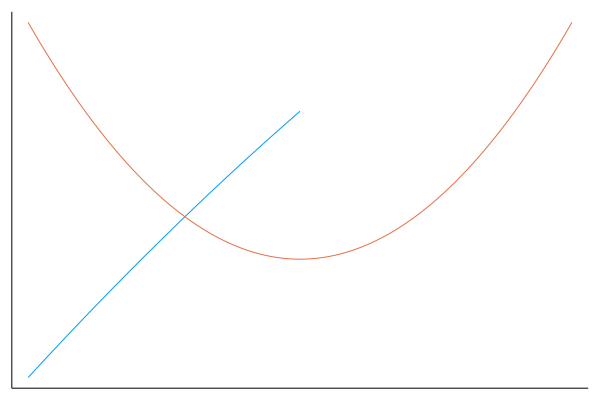
\includegraphics[]{images/bezint-2:1.png}}
    child{
      node [] {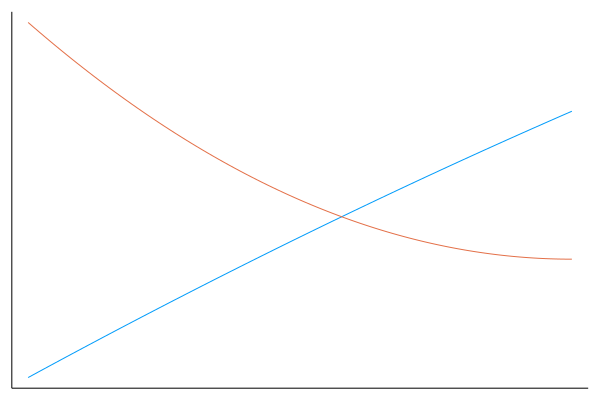
\includegraphics[]{images/bezint-3:1, 3.png}}
      child{
        node [] {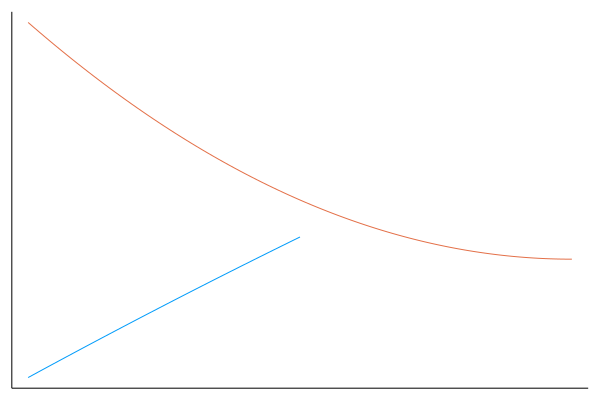
\includegraphics[]{images/bezint-4:1, 3, 1.png}}
        child{
          node [] {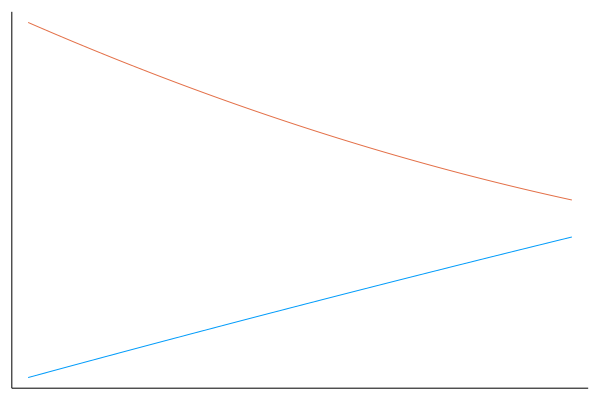
\includegraphics[]{images/bezint-5:1, 3, 1, 3.png}}
        }
        child{
          node [] {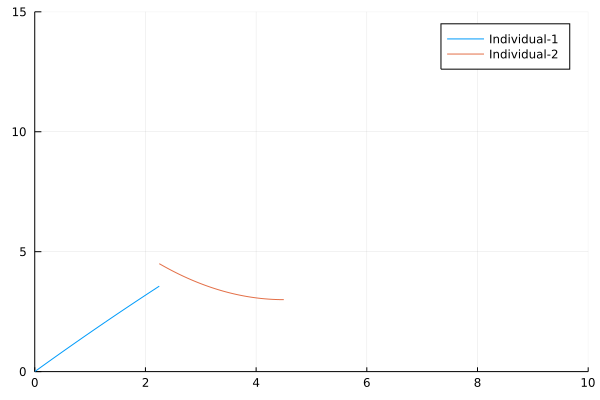
\includegraphics[]{images/bezint-5:1, 3, 1, 4.png}}
          child{
            node [] {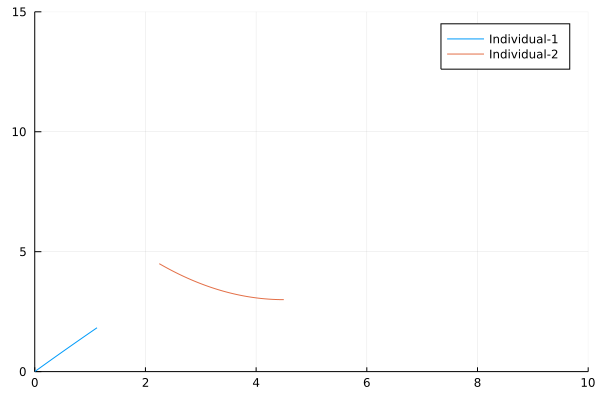
\includegraphics[]{images/bezint-6:1, 3, 1, 4, 1.png}}
          }
          child{
            node [] {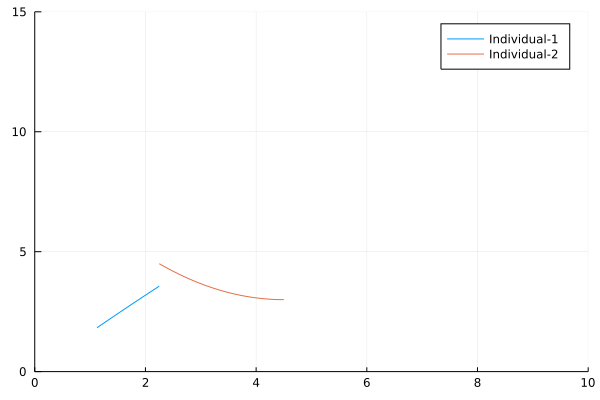
\includegraphics[]{images/bezint-6:1, 3, 1, 4, 2.png}}
            child{
              node [] {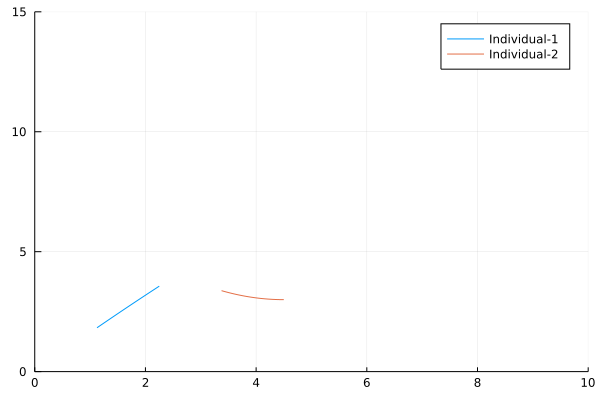
\includegraphics[]{images/bezint-7:1, 3, 1, 4, 2, 3.png}}
            }
            child{
              node [] {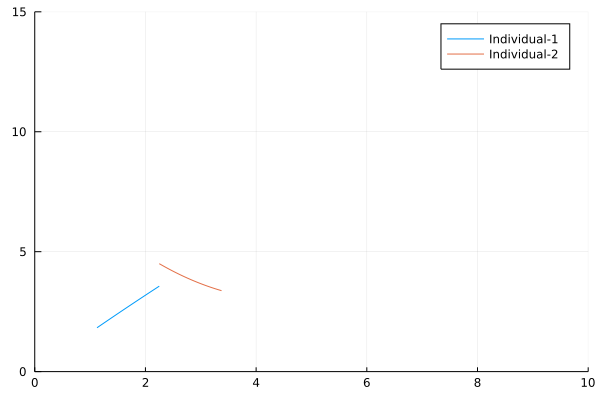
\includegraphics[]{images/bezint-7:1, 3, 1, 4, 2, 4.png}}
              child{
                node [] {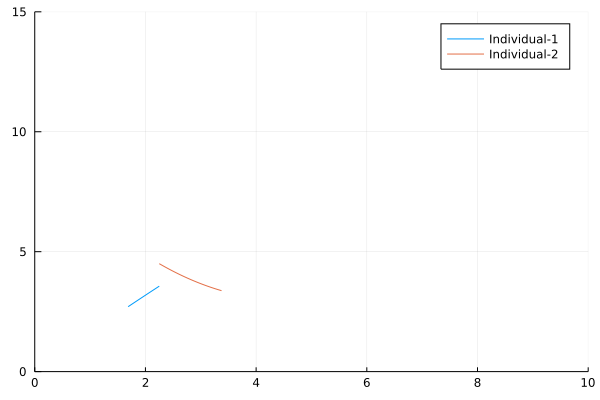
\includegraphics[]{images/bezint-8:1, 3, 1, 4, 2, 4, 1.png}}
              }
              child{
                node [] {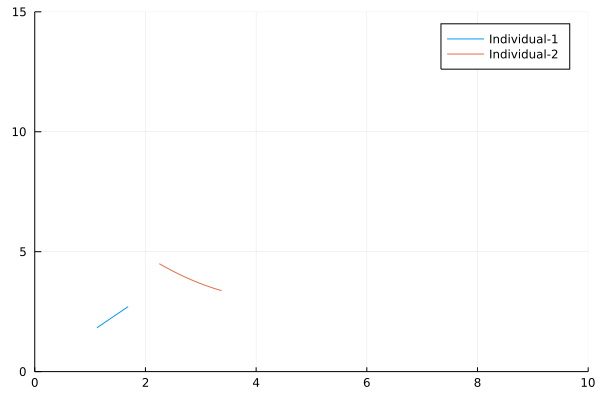
\includegraphics[]{images/bezint-8:1, 3, 1, 4, 2, 4, 2.png}}
              }
            }
          }
        }
      }
      child{
        node [] {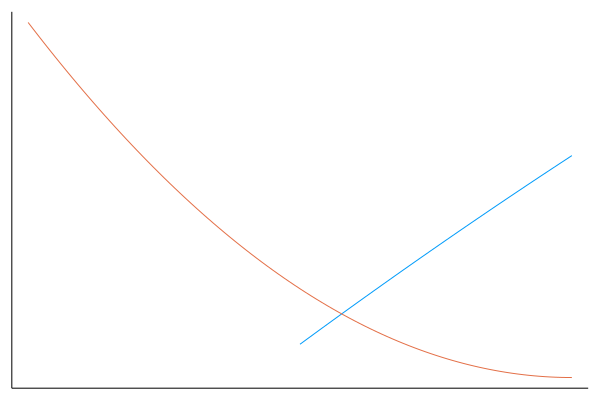
\includegraphics[]{images/bezint-4:1, 3, 2.png}}
        child{
          node [] {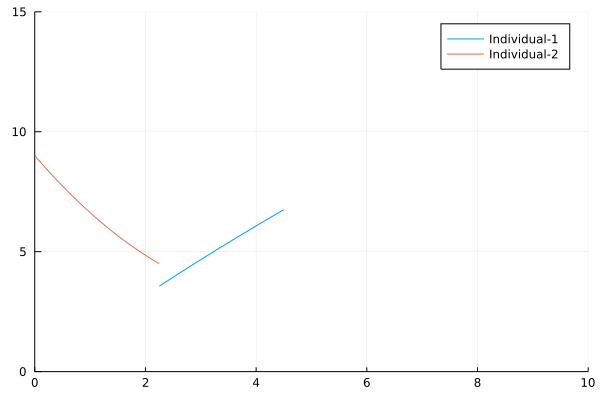
\includegraphics[]{images/bezint-5:1, 3, 2, 3.png}}
          child{
            node [] {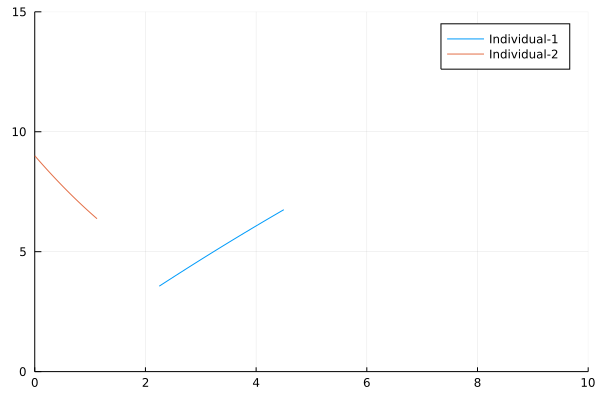
\includegraphics[]{images/bezint-6:1, 3, 2, 3, 3.png}}
          }
          child{
            node [] {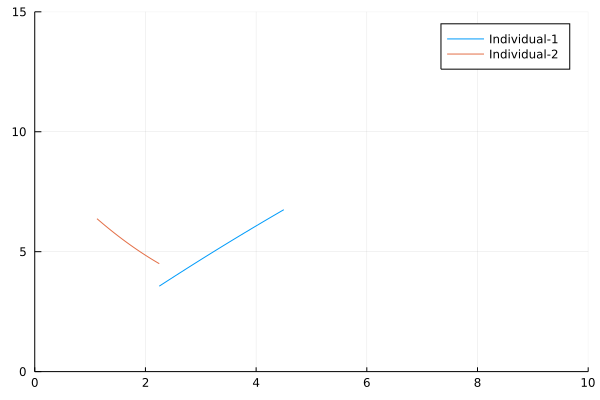
\includegraphics[]{images/bezint-6:1, 3, 2, 3, 4.png}}
            child{
              node [] {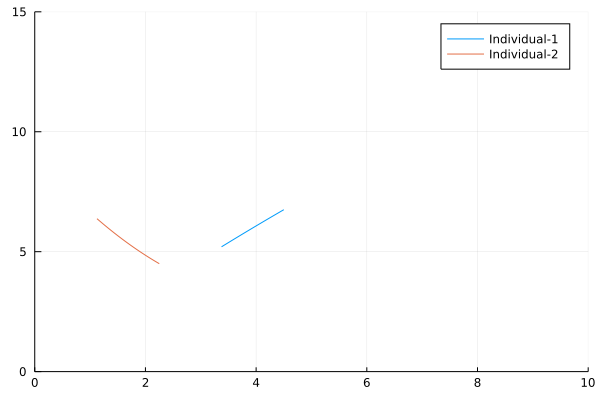
\includegraphics[]{images/bezint-7:1, 3, 2, 3, 4, 1.png}}
            }
            child{
              node [] {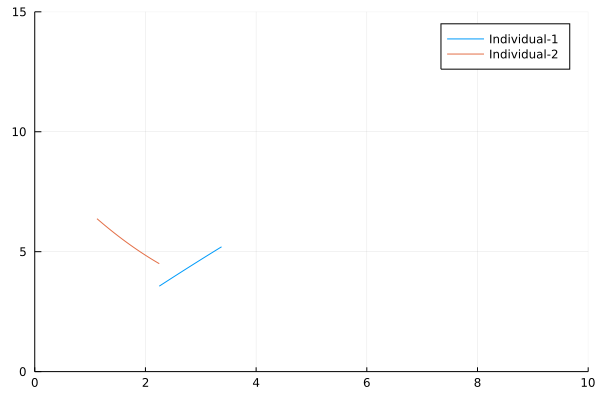
\includegraphics[]{images/bezint-7:1, 3, 2, 3, 4, 2.png}}
              child{
                node [] {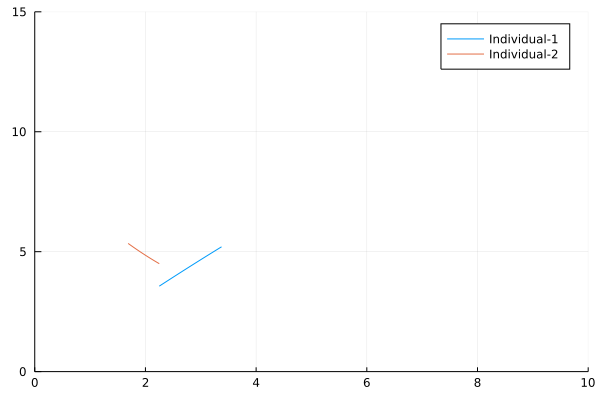
\includegraphics[]{images/bezint-8:1, 3, 2, 3, 4, 2, 3.png}}
              }
              child{
                node [] {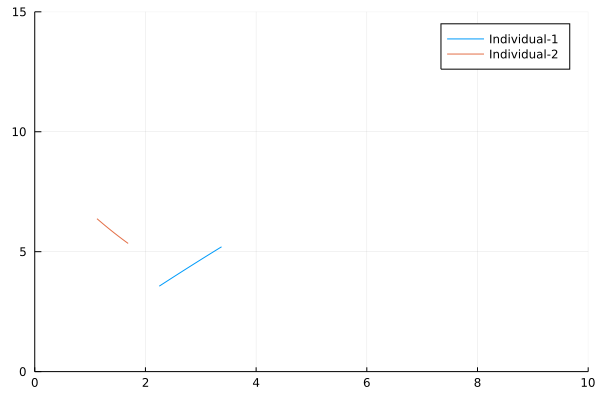
\includegraphics[]{images/bezint-8:1, 3, 2, 3, 4, 2, 4.png}}
              }
            }
          }
        }
        child{
          node [] {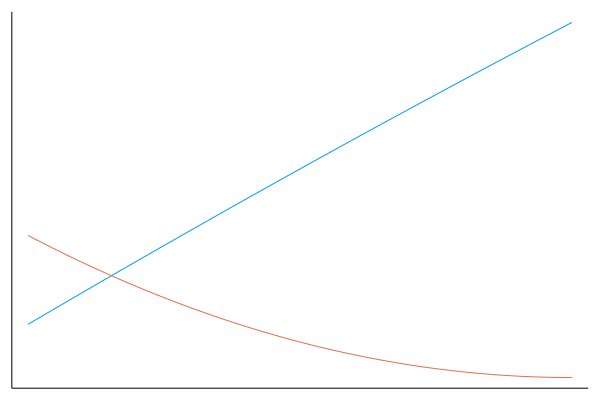
\includegraphics[]{images/bezint-5:1, 3, 2, 4.png}}
          child{
            node [] {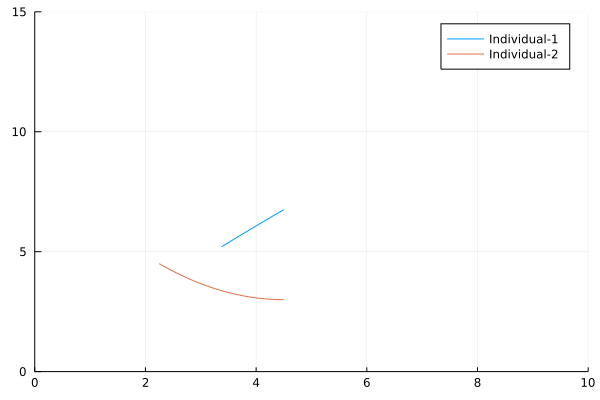
\includegraphics[]{images/bezint-6:1, 3, 2, 4, 1.png}}
          }
          child{
            node [] {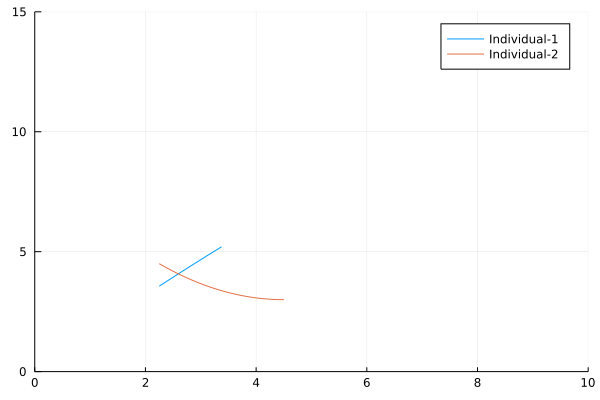
\includegraphics[]{images/bezint-6:1, 3, 2, 4, 2.png}}
            child{
              node [] {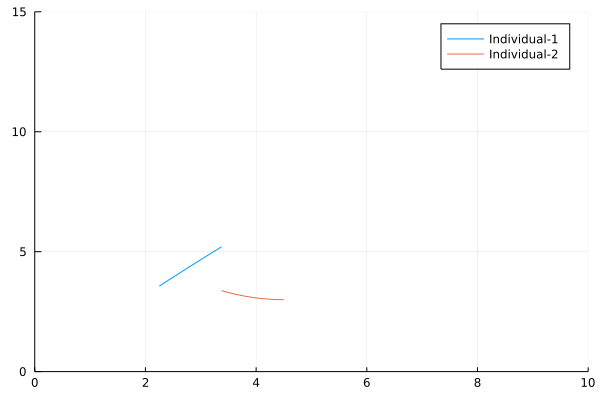
\includegraphics[]{images/bezint-7:1, 3, 2, 4, 2, 3.png}}
            }
            child{
              node [] {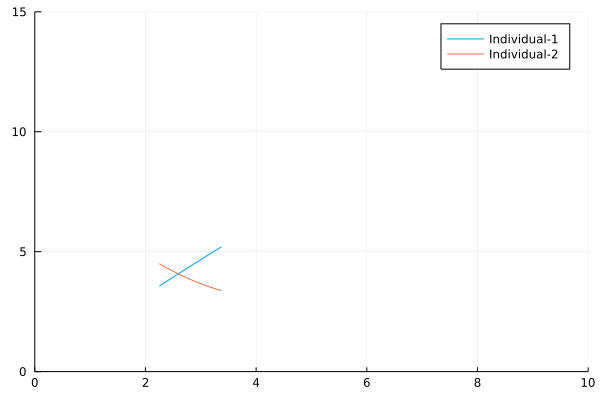
\includegraphics[]{images/bezint-7:1, 3, 2, 4, 2, 4.png}}
            }
          }
        }
      }
    }
    child{
      node [] {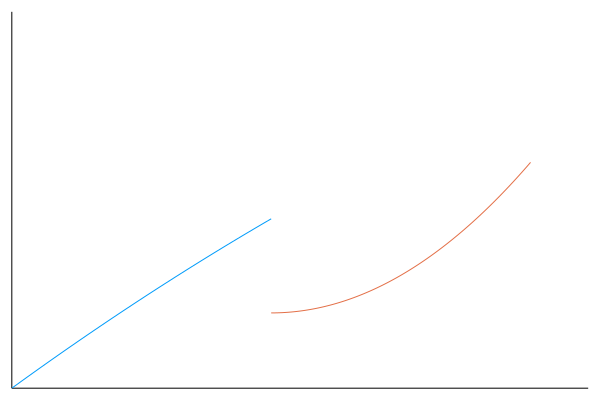
\includegraphics[]{images/bezint-3:1, 4.png}}
      child{
        node [] {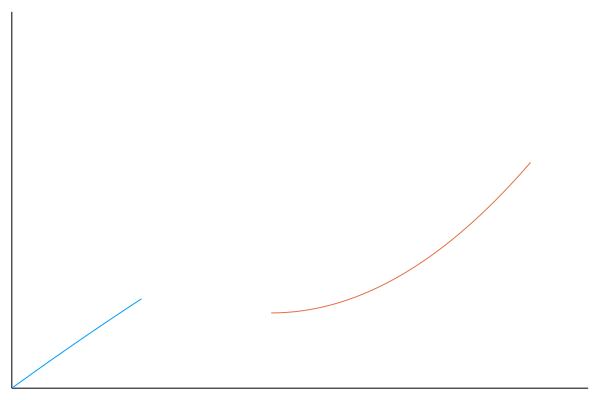
\includegraphics[]{images/bezint-4:1, 4, 1.png}}
      }
      child{
        node [] {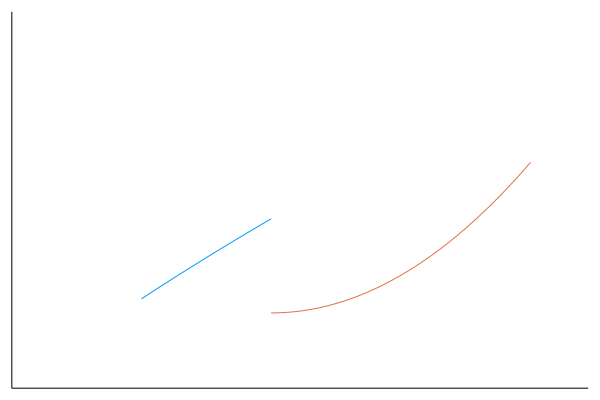
\includegraphics[]{images/bezint-4:1, 4, 2.png}}
        child{
          node [] {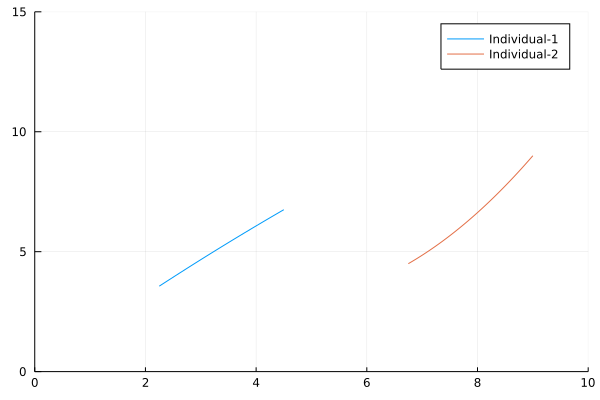
\includegraphics[]{images/bezint-5:1, 4, 2, 3.png}}
        }
        child{
          node [] {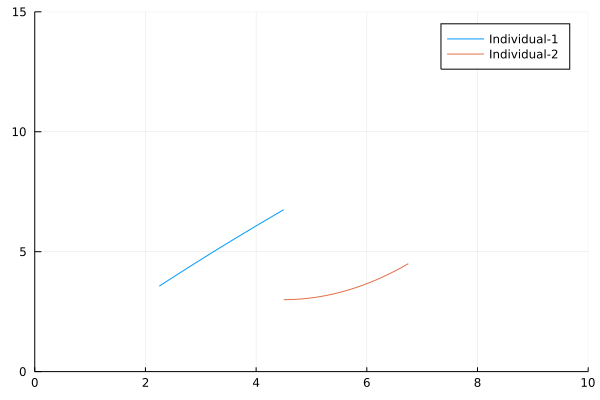
\includegraphics[]{images/bezint-5:1, 4, 2, 4.png}}
          child{
            node [] {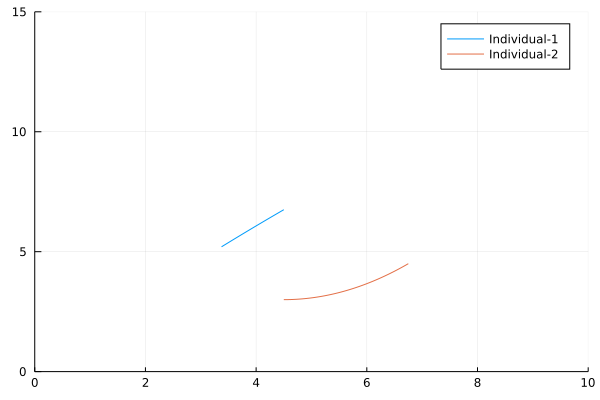
\includegraphics[]{images/bezint-6:1, 4, 2, 4, 1.png}}
          }
          child{
            node [] {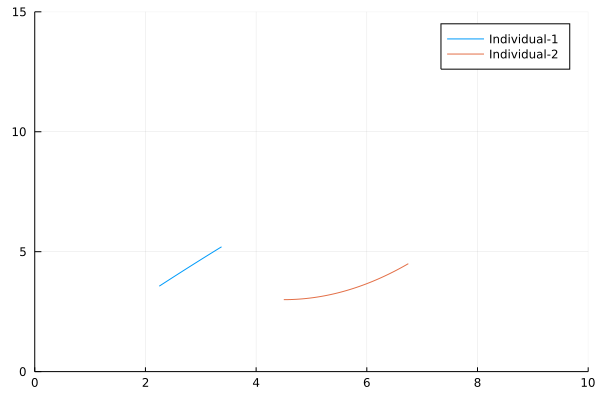
\includegraphics[]{images/bezint-6:1, 4, 2, 4, 2.png}}
          }
        }
      }
    }
}
  child{
    node [] {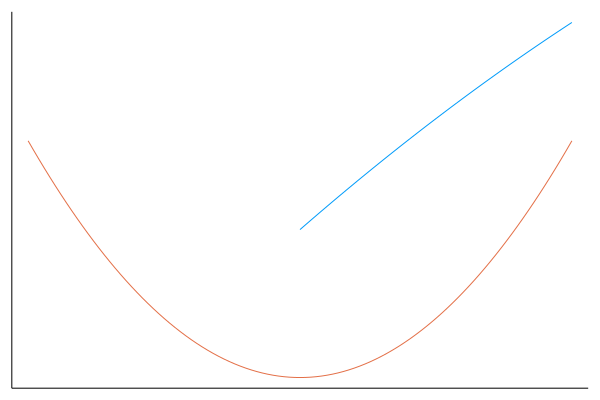
\includegraphics[]{images/bezint-2:2.png}}
    child{
      node [] {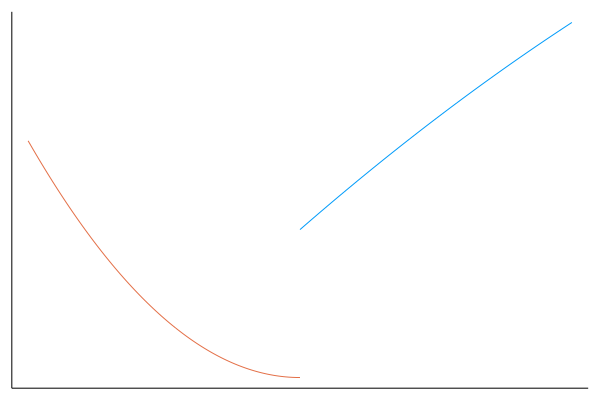
\includegraphics[]{images/bezint-3:2, 3.png}}
      child{
        node [] {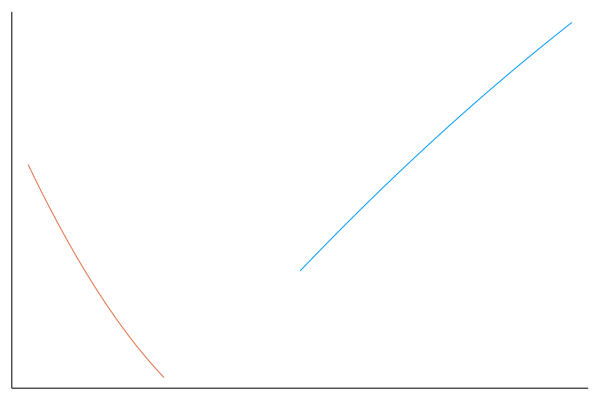
\includegraphics[]{images/bezint-4:2, 3, 3.png}}
      }
      child{
        node [] {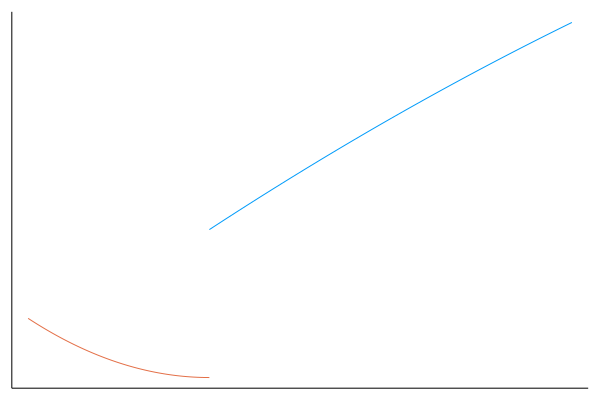
\includegraphics[]{images/bezint-4:2, 3, 4.png}}
      }
    }
    child{
      node [] {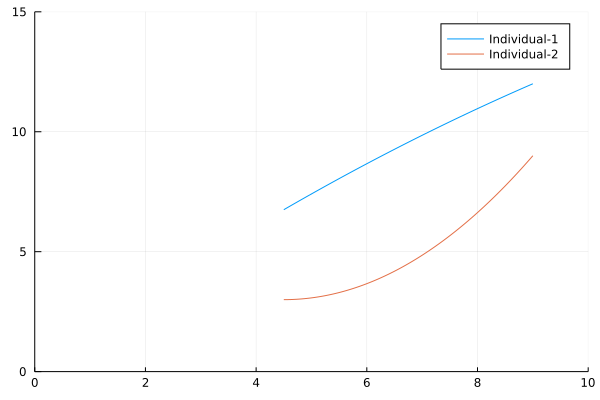
\includegraphics[]{images/bezint-3:2, 4.png}}
      child{
        node [] {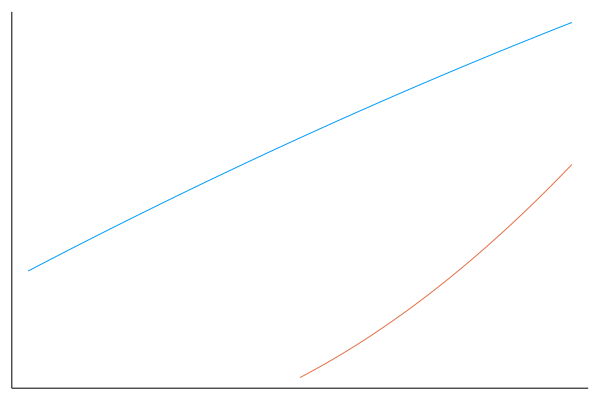
\includegraphics[]{images/bezint-4:2, 4, 3.png}}
        child{
          node [] {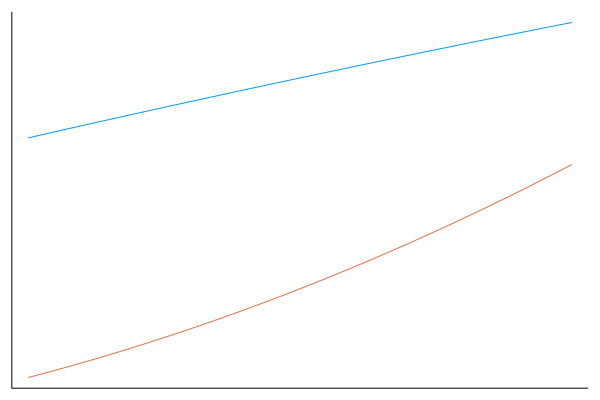
\includegraphics[]{images/bezint-5:2, 4, 3, 1.png}}
        }
        child{
          node [] {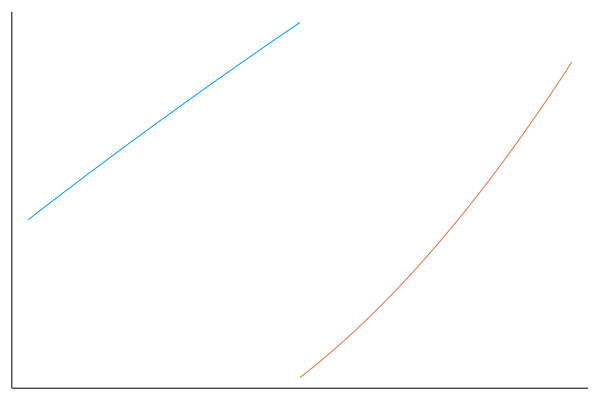
\includegraphics[]{images/bezint-5:2, 4, 3, 2.png}}
          child{
            node [] {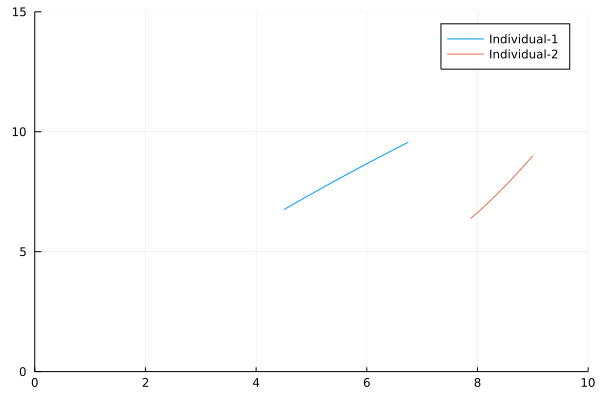
\includegraphics[]{images/bezint-6:2, 4, 3, 2, 3.png}}
          }
          child{
            node [] {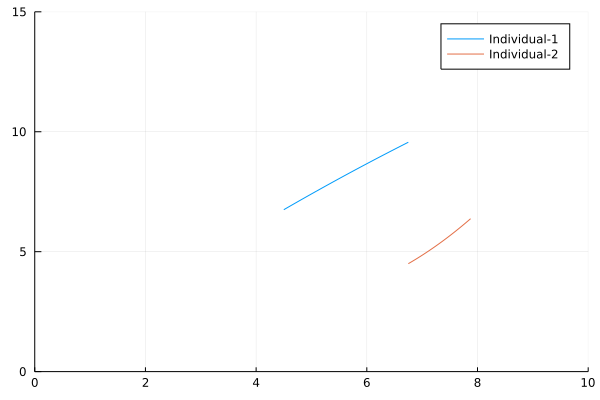
\includegraphics[]{images/bezint-6:2, 4, 3, 2, 4.png}}
          }
        }
      }
      child{
        node [] {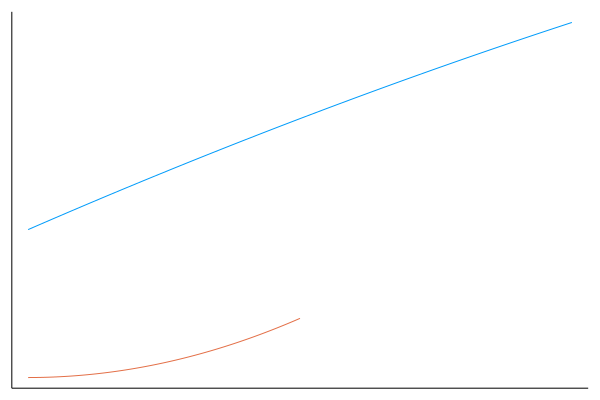
\includegraphics[]{images/bezint-4:2, 4, 4.png}}
      }
    }
  }
  ;

%  \node [below left = of p2-1] (p3-13) {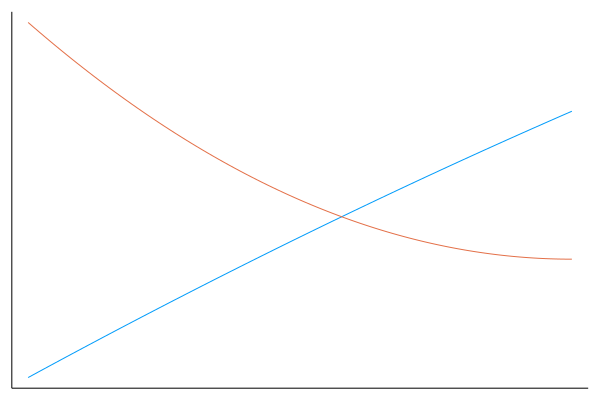
\includegraphics[]{images/bezint-3:1, 3.png}};
%  \node [below right = of p2-1] (p3-14) {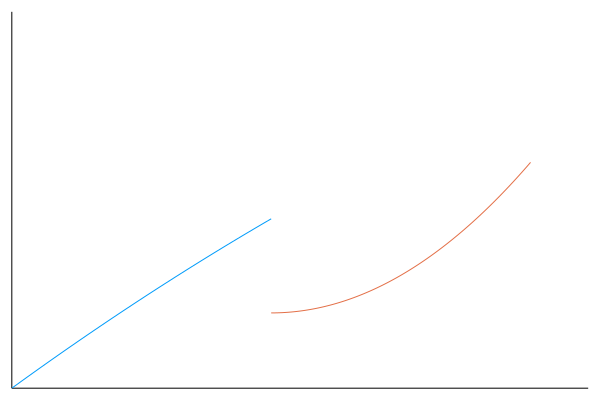
\includegraphics[]{images/bezint-3:1, 4.png}};
%
%  \node [below left = of p2-2] (p3-23) {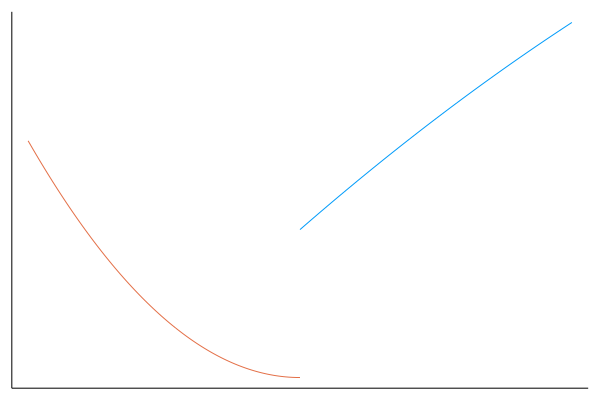
\includegraphics[]{images/bezint-3:2, 3.png}};
%  \node [below right = of p2-2] (p3-24) {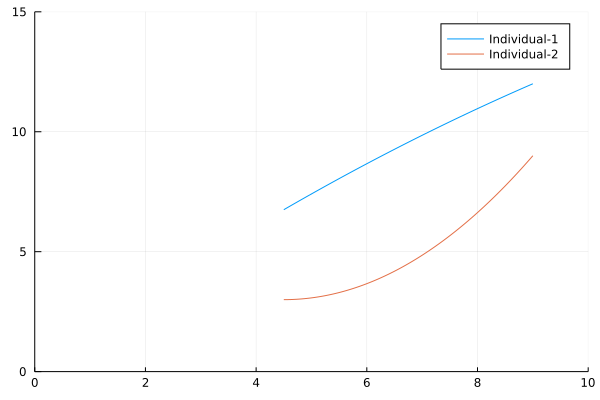
\includegraphics[]{images/bezint-3:2, 4.png}};


\end{tikzpicture}

\end{document}
